
\title{Lab Report 05 - Image Segmentation}
\author{
        Manuel Galliker  14-921-969 \\
                manuelga@student.ethz.ch
}
\date{\today}

\documentclass[12pt]{article}
\usepackage{graphicx}
\begin{document}
\maketitle


\section{1. Image Preprocessing}

\vspace{5mm}
\begin{figure}[ht]
	\centering
	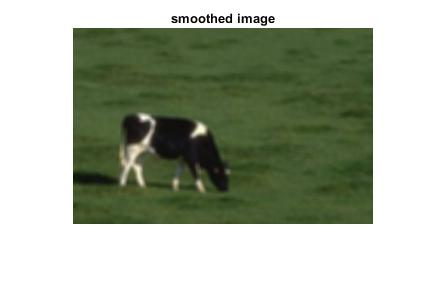
\includegraphics[width=0.9\textwidth]{smooth.jpg}
	\caption{Smooth Image}
	\label{fig1}
\end{figure}
\vspace{5mm}
\begin{figure}[ht]
	\centering
	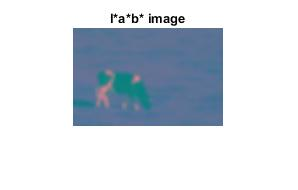
\includegraphics[width=0.9\textwidth]{lab.jpg}
	\caption{Smooth L-a-b Image}
	\label{fig1}
\end{figure}
\vspace{5mm}


Before doing the image segmentation the images have to be gaussian filtered and converted to the $L*a*b$ space. For the smoothing a 5x5 gaussian filter with $\sigma = 5$ was used. For the Image segmentation the $L*a*b$ space is preferable. This space consists of a lightness value $L$ and the colour values $a$ and $b$. It can therefore decouple the brithness from the colour space, which gives a better robustness for different lightning conditions. This was done using the matlab functions $makecform$ and $applycform$.  



\section{Mean-Shift Segmentation}

\vspace{5mm}
\begin{figure}[ht]
	\centering
	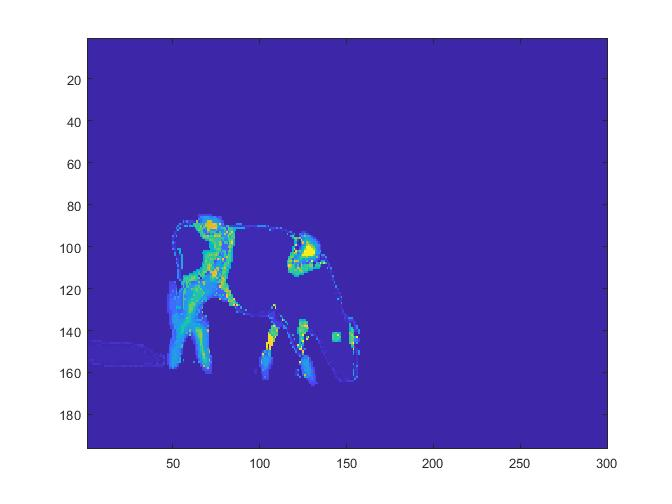
\includegraphics[width=0.9\textwidth]{r5p163a.jpg}
	\caption{Mean-Shift Image 4: R = 5, thr = 2.5, 163 peaks}
	\label{fig1}
\end{figure}
\vspace{5mm}
\begin{figure}[ht]
	\centering
	
\includegraphics[width=0.9\textwidth]{r5p163b.jpg}
	\caption{Mean-Shift Image 5: R = 5, thr = 2.5, 163 peaks}
	\label{fig1}
\end{figure}
\vspace{5mm}
\begin{figure}[ht]
	\centering
	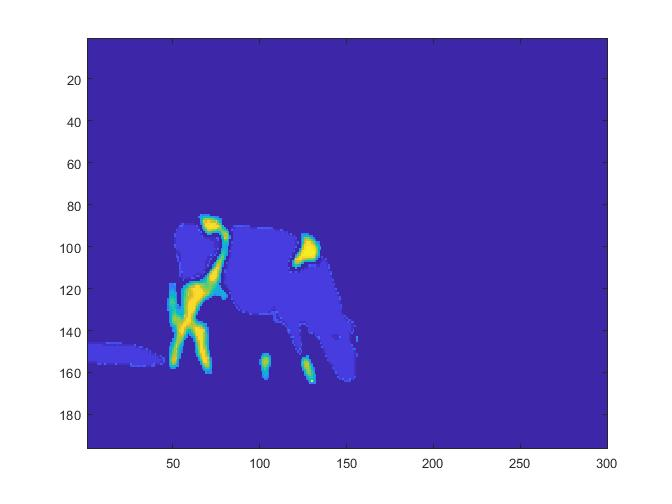
\includegraphics[width=0.9\textwidth]{r10p25a.jpg}
	\caption{Mean-Shift Image 4: R = 10, thr = 5, 25 peaks}
	\label{fig1}
\end{figure}
\vspace{5mm}
\begin{figure}[ht]
	\centering
	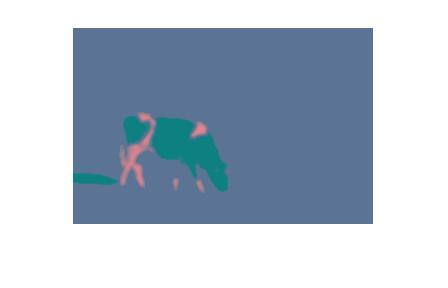
\includegraphics[width=0.9\textwidth]{r10p25b.jpg}
	\caption{Mean-Shift Image 5: R = 10, thr = 5, 25 peaks}
	\label{fig1}
\end{figure}
\vspace{5mm}

The Mean-Shift Segmentation repeatedly calculates of all the pixels withing a certain radius $r$ around a point. It does this until the nest shift is below a certain threshhold.



It is intuitivly clear and could be validated that increasing the radius is computationally more expensive and takes more time. Therefore, the radius should be choosen only large enough to fullfil any time based constraints for the desired application for this computationally expensive algorithm. 
 




\section{EM Segmentation}
The last part of this exercise is the EM implementation. Here the following parameters are used: 
\vspace{5mm}
\newline
K: Number of clusters
\vspace{5mm}
\newline
$\alpha = 1/K$: equal weighting
\vspace{5mm}
\newline
$\Sigma$: 3x3 matrix corresponding to the range of $L*a*b$ space
\vspace{5mm}
\newline
$\mu$: equally spread over the $L*a*b$ space

The implementet fuctions $expectation$ and $maximization$ evaluate the probability and update the parameters respectivly. 

$ mu = \left[ \begin{array}{rrr}
   42.2449 & 137.6082  & 89.1000\\
123.5445 & 125.2056 & 114.4193\\
137.0442 & 140.5672 & 149.0963\\
\end{array}\right] $
\vspace{5mm}
$ sigma1 = \left[ \begin{array}{rrr}
  819.2520 &-137.2637 & 238.9867\\
-137.2637 &  33.0107  &-47.3915\\
238.9867 & -47.3915  & 79.1724\\
\end{array}\right] $
\vspace{5mm}
$ sigma2 = 1.0e+03 *\left[ \begin{array}{rrr}
    2.3539 &   0.0715 &   0.0406\\
0.0715  &  0.0115  & -0.0069\\
0.0406  & -0.0069 &   0.0242\\
\end{array}\right] $
\vspace{5mm}
$ sigma3 = \left[ \begin{array}{rrr}
   56.7097 &   0.3528 &   0.4147\\
0.3528  &  0.8359  & -0.1712\\
0.4147 &  -0.1712  &  1.5366\\
\end{array}\right] $
\vspace{5mm}
$ sigma3 = \left[ \begin{array}{rrr}
0.1061  &  0.0377  &  0.8562\\
\end{array}\right] $



\vspace{5mm}
\begin{figure}[ht]
	\centering
	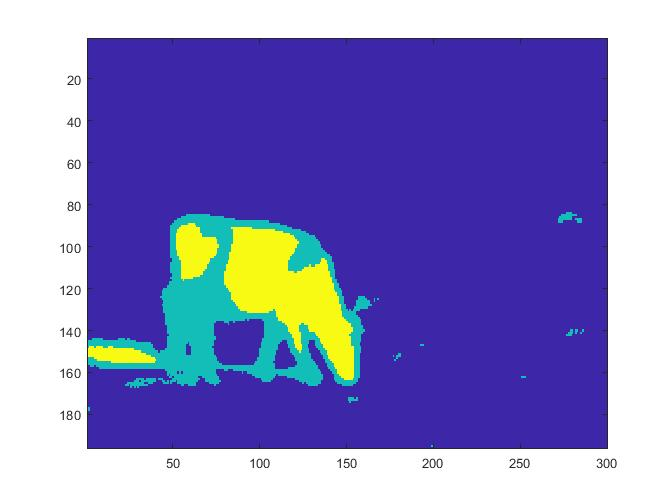
\includegraphics[width=0.9\textwidth]{k3_22a.jpg}
	\caption{EM Image 4: K = 3}
	\label{fig1}
\end{figure}
\vspace{5mm}
\begin{figure}[ht]
	\centering
	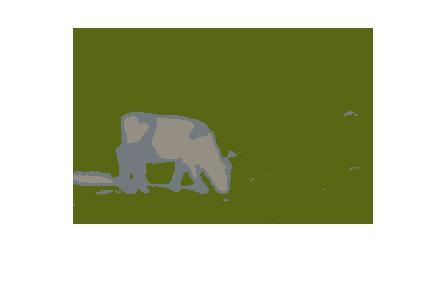
\includegraphics[width=0.9\textwidth]{k3_22b.jpg}
	\caption{EM Image 5: K = 3}
	\label{fig1}
\end{figure}
\vspace{5mm}



\end{document}